\documentclass[14pt, a4paper]{extarticle}
\usepackage{style}
\usepackage{array}
\usepackage{biblatex}
\usepackage{amsmath}
\usepackage{amssymb}
\usepackage{amsthm}
\usepackage{indentfirst}
\usepackage{listings}
\usepackage{xcolor}
\usepackage{fefutitle}
\usepackage[justification=centering]{caption}
\usepackage{float}
\usepackage{geometry}
\usepackage{framed}

\let\oldref\ref
\renewcommand{\ref}[1]{(\oldref{#1})}
\newgeometry{top=2cm, bottom=2cm, right=15mm, left=25mm}
\setlength{\baselineskip}{15pt}
\renewcommand\qedsymbol{$\blacksquare$}

\begin{document}
	
	\fefutitle{2}{Решение краевой задачи для уравнение Лапласа в круге и вне круга методом Фурье. Формула Пуассона решения краевой задачи для уравнения Лапласа в круге и вне круга.}
	\pagebreak
	
	\section{Введение}
		При исследовании стационарных процессов  обычно приходят к уравнения эллиптического вида.[2, c. 295] К эллиптическому виду относится уравнение Лапласа
		\begin{equation*}
			\Delta u = 0, 
		\end{equation*}
		где $\Delta$ -- оператор Лапласа. В n-мерном пространстве выглядит следующим образом
		\begin{equation}
			\Delta u = \dfrac{\partial^2 u}{\partial x^2_1} + \dfrac{\partial^2 u}{\partial x^2_2} + ... +   \dfrac{\partial^2 u}{\partial x^2_n}. 
		\end{equation}
		
		Чтобы выделить единственное решение уравнение Лапласа необходимо поставить одно из граничных условий:
		\begin{enumerate}
			\item $u = g$ на $\Gamma$ -- условие Дирихле,
			\item $\dfrac{\partial u}{\partial n} = g$ на $\Gamma$ -- условие Неймана,
			\item $\dfrac{\partial u}{\partial n}  + \alpha u = g$ на $\Gamma$ -- условие 3-го рода,
			\item $ \alpha u + \beta\dfrac{\partial u}{\partial n}  = g$ на $\Gamma$ -- смешанное.
		\end{enumerate}
		
		Решение краевых задач может быть найдено методом Фурье в случае некоторых простейших областей(круг, промоугольник, шар и др.).[2] В этом реферате мы рассмотрим решение задачи Дирихле для уравнения Лапласа в круге и вне круга.

	\section{Основная часть}
		\subsection{Постановка краевых задач. Применение метода Фурье.}
		Пусть $\Omega = \Omega_a = \{ (x, y) \in \mathbb{R}^2 : x^2 + y^2 < a^2 \}$ -- круг радиуса $a$, $\Omega_e = \mathbb{R} \setminus \overline{\Omega}$.
		Рассмотрим две задачи[1]:
		\begin{enumerate}
			\item Внутренная задача Дирихле, заключающаяся в нахождении классического решения $u$ уравнения Лапласа
				     \begin{equation} \label{1} \Delta u = 0 \end{equation}  
				     в $\Omega$, удовлетворяющего граничному условию
					 \begin{equation} u\big|_{\text{Г}} = g  \label{2}  \end{equation}
			\item Внешняя задача Дирихле, заключающаяся в нахождении классического решения уравнения  \ref{1}  в области $\Omega_e$, удовлетворяющего граничному условию \ref{2} и условию на бесконечности:
				\begin{equation}
					u(x, y) = O(1)\: \text{при} \: (x^2+y^2)  \rightarrow \inf
				\end{equation}
				
		\end{enumerate}
		Для решения этих задач перейдем в полярные координаты[3]
		\begin{equation}
			\begin{cases}
				x = r\cos{\varphi}\\
				y = r\sin{\varphi}
			\end{cases}
		\end{equation}
		Уравнение \ref{1} в полярных координатах имеет вид[1]:
		\begin{equation}
			\Delta u = \dfrac{1}{\rho} \dfrac{\partial}{\partial \rho} \bigg( \rho \dfrac{\partial u}{\partial \rho} \bigg) + \dfrac{1}{\rho^2} \dfrac{\partial^2 u}{\partial \varphi^2} = 0 \label{5}
		\end{equation}
		Решим задачу методом разделения переменных, т.е. будем искать частное решение уравнения \ref{1} в виде
		\begin{equation}
			u(\rho, \varphi) = R(\rho)\Phi(\varphi)	\label{6}
		\end{equation}
		Подставляя \ref{6} в \ref{5} и разделяя переменные получаем
		\begin{equation}
			\dfrac{\rho(\rho R')'}{R} = - \dfrac{\Phi''}{\Phi} = \lambda,
		\end{equation}
		где $\lambda = const$. 
		
		\begin{framed}
			\begin{quote}
				\textit{\textbf{Комментарий:}} 
				
				\textit{В разных частях полученного равенства стоят функции разных переменных.
					Это может быть только тогда, когда обе они постоянны.}
			\end{quote}
		\end{framed}
		
		Отсюда получаем два обыкновенных дифференциальных уравнения
		\begin{equation}
			\rho^2 R'' + \rho R' - \lambda R = 0 \label{8}
		\end{equation}
		\begin{equation}
			\Phi'' + \lambda \Phi = 0 \label{9}
		\end{equation}
		Заметим, что при измении угла $\varphi$ на величину $2\pi$ однозначная функция $u(\rho, \varphi)$ должна вернуться к исходному значению.
		\begin{equation}
			u(\rho, \varphi) = u(\rho, \varphi + 2\pi)
		\end{equation}
		Отсюда следует, что 
		\begin{equation}
			\Phi(\varphi) = \Phi(\varphi + 2\pi) \label{11}
		\end{equation}
		Равенства \ref{9} и \ref{11} представляют собой спектральную задачу. Ее решение имеет вид
		\begin{equation}
			\lambda_k = k^2, \; \Phi_k(\varphi) = a_k\cos(k\varphi) + b_k\sin(k\varphi), k = 0,1,2...
		\end{equation}
		\begin{framed}
			\begin{quote}
		\textit{\textbf{Комментарий:}}
		
			\textit{Составим и решим характеристическое уравнение
			\begin{equation*}
				z^2 + \lambda = 0
			\end{equation*}
			\begin{equation*}
				z = \pm \sqrt{-\lambda}
			\end{equation*}
			Рассмотрим разные знаки $\lambda$
			\begin{enumerate}
				\item$ \lambda$ < 0
				\begin{equation*}
					\Phi(\varphi) = a e^{\sqrt{-\lambda}\varphi} + b e^{-\sqrt{-\lambda}\varphi}
				\end{equation*}
				В данном случае задача имеет только тривиальное решение.
				\item $\lambda$ = 0
				\begin{equation*}
					\Phi(\varphi) = a + b\varphi
				\end{equation*}
				При $b = 0$ получаем периодическую функцию -- константу.
				\item $\lambda$ > 0
				\begin{equation*}
					\Phi(\varphi) = a \cos{\sqrt{\lambda}\varphi}+ b \sin{\sqrt{\lambda}\varphi}
				\end{equation*}
				При $\lambda= k^2$ -- функция периодическая.
				Решения из пункта 2 и 3 можно объединить, если считать, что $k$ меняется, начиная с $0$.[3]
			\end{enumerate}
			Проверим:\\
			\begin{minipage}{0.45\textwidth}
				\begin{equation*}
					(\cos{\sqrt{\lambda}\varphi})'' = -\lambda \cos{\sqrt{\lambda}\varphi}
				\end{equation*}
				\begin{equation*}
					-\lambda \cos{\sqrt{\lambda}\varphi} + \lambda \cos{\sqrt{\lambda}\varphi} = 0
				\end{equation*}
			\end{minipage}
			\hfill
			\begin{minipage}{0.45\textwidth}
				\begin{equation*}
					(\sin{\sqrt{\lambda}\varphi})'' = -\lambda \sin{\sqrt{\lambda}\varphi}
				\end{equation*}
				\begin{equation*}
					-\lambda \sin{\sqrt{\lambda}\varphi} + \lambda \sin{\sqrt{\lambda}\varphi} = 0
				\end{equation*}
			\end{minipage}\\
			Оба решения удовлетворяют уравнению, а так как оно однородное, то и их линейная комбинация тоже является решением.}
			\end{quote}
			\end{framed}
			
			Перейдем к решению уравнения \ref{8}. Заменим $\lambda$ на $k^2$. Получим уравнение Эйлера.[1]
			\begin{equation}
					\rho^2 R'' + \rho R' - k^2 R = 0 \label{13}
			\end{equation}
			Полагая $R(\rho) = \rho^\mu$, находим при $k > 0$ два решения: $\rho^k$ и $\rho^{-k}$, при $k = 0$ решениями являются $1$ и $\ln{\rho}$.
			
			\begin{framed}
				\begin{quote}
			\textit{\textbf{Комментарий:}}
			
			\textit{
			\begin{minipage}{0.2\textwidth}
				$R(\rho) = \rho^\mu$
			\end{minipage}
			\hfill
			\begin{minipage}{0.25\textwidth}
				$R'(\rho) = \mu \rho^{(\mu-1)}$
			\end{minipage}
			\hfill
			\begin{minipage}{0.3\textwidth}
				$R''(\rho) = \mu(\mu - 1) \rho^{(\mu-2)}$
			\end{minipage}\\
			Подставляем в \ref{13} и сокращая на $\rho^\mu$, получаем
			\begin{equation*}
				\mu^2 = k^2 \Rightarrow \mu = \pm k
			\end{equation*}
			При $k > 0$ получаем общее решение:
			\begin{equation*}
				R(\rho) = a \rho^k + b \rho^{-k}
			\end{equation*}
			Проверка:\\
			\begin{minipage}{0.45\textwidth}
				\[ R' = k \rho^{k-1} \]
				\[ R'' = k(k-1) \rho^{k-2} \]
				\[ k(k-1) \rho^k + k\rho^k - k^2\rho^k = 0 \]
				\[ k^2 - k  + k - k^2 = 0 \]
			\end{minipage}
			\hfill
			\begin{minipage}{0.45\textwidth}
				\[ R' = -k \rho^{-k-1} \]
				\[ R'' = -k(-k-1) \rho^{-k-2} \]
				\[ -k(k-1) \rho^k - k\rho^k - k^2\rho^k = 0 \]
				\[ k^2 + k  - k - k^2 = 0 \]
			\end{minipage}\\
			При $k = 0$ получаем общее решение:
			\[ R(\rho) = a + b \ln{\rho} \]
						Проверка:\\
			\begin{minipage}{0.45\textwidth}
				\[ R' = 0 \]
				\[ R'' =0\]
				\[ 0 = 0 \]
			\end{minipage}
			\hfill
			\begin{minipage}{0.45\textwidth}
				\[ R' = \dfrac{1}{\rho}\]
				\[ R'' = -\dfrac{1}{\rho^2} \]
				\[ -1 + 1 = 0 \]
			\end{minipage}\\
			}
			\end{quote}
			\end{framed}
			
			Для внутренней задачи возьмем[1]
			\begin{equation}
				R_0(\rho) = 1,\: R_k(\rho) = \rho^k, k \geq 1
			\end{equation}
			и для внешней
						\begin{equation}
				R_0(\rho) = 1,\: R_k(\rho) = \rho^{-k}, k \geq 1
			\end{equation}
			Итак, частные решения найдены:
			\begin{equation}
				u_k(\rho, \varphi) = \rho^k(a_k \cos{k\varphi} + b_k \sin{k\varphi}), k = 0, 1, 2...  \label{16}
			\end{equation}
			для внутренней задачи Дирихле и
						\begin{equation}
				u_k(\rho, \varphi) = \rho^{-k}(a_k \cos{k\varphi} + b_k \sin{k\varphi}), k = 0, 1, 2... \label{17}
			\end{equation}
			для внешней задачи Дирихле.
			
			\begin{framed}
				\begin{quote}
			\textit{\textbf{Комментарий:}}
			
			\textit{
				Найдем частные производные \ref{16} по $\rho$ и $\varphi$ и подставим в \ref{5}.\\
					\[ \dfrac{\partial u}{\partial \rho} = k  \rho^{(k-1)} (a_k \cos{k\varphi} + b_k \sin{k\varphi}) \]
					\[ \dfrac{\partial}{\partial \rho} \bigg(  \rho \dfrac{\partial u}{\partial \rho} \bigg) = k^2 \rho^{(k-1)}  (a_k \cos{k\varphi} + b_k \sin{k\varphi}) \]
					\[ \dfrac{\partial u}{\partial \varphi} = k \rho^k ( - a_k \sin{k\varphi} + b_k \cos{k\varphi} ) \]
					\[ \dfrac{\partial^2 u}{\partial \varphi^2} = - k^2 \rho^k (a_k \cos{k\varphi} + b_k \sin{k\varphi}) \]
				\[  k^2 \rho^{(k-2)}  (a_k \cos{k\varphi} + b_k \sin{k\varphi})  -  k^2 \rho^{k-2} (a_k \cos{k\varphi} + b_k \sin{k\varphi}) = 0\]
				Получили тождество, значит полученое решение верно. Аналогично и для решения \ref{17} внешней задачи.
			}
						\end{quote}
			\end{framed}
			
			Бесконечные суммы этих решений[1]
			\begin{equation}
				u(\rho, \varphi) =  \sum_{0}^{\infty} \rho^k(a_k \cos{k\varphi} + b_k \sin{k\varphi}) \label{18}
			\end{equation}
			\begin{equation}
				u(\rho, \varphi) =  \sum_{0}^{\infty} \rho^{-k}(a_k \cos{k\varphi} + b_k \sin{k\varphi}) \label{19}
			\end{equation}
			также будут гармоническими функциями, при условии, что ряд \ref{18} (либо \ref{19}) можно почленно дифференцировать по $r$ и по $\varphi$ с сохранением равномерной сходимости в $\Omega$($\Omega_e$).
			
			Для определения коэффициентов $a_k$ и $b_k$ воспользуемся граничным условием \ref{2}.
			\begin{equation}
				u(a, \varphi) = \sum_{0}^{\infty} a^k (a_k \cos{k\varphi} + b_k \sin{k\varphi)} \label{20}
			\end{equation}
			Предположим, что функция $g$ удовлетворяет условиям
			
			 (i) $g \in C^{0}[0, 2\pi], g(0) = g(2\pi)$
			 С учетом условий (i) функцию $g$ можно разложить в ряд Фурье:
			 \begin{equation}
			 	g(\varphi) = \dfrac{\alpha_0}{2} + \sum_{1}^{\infty} (\alpha_k \cos{k\varphi} + \beta_k \sin{k\varphi}), \label{21}
			 \end{equation}
			 где коэффициенты $\alpha_0$, $\alpha_k$ и $\beta_k$ определяются формулами
			 \begin{equation}
     		 	\alpha_0 = \dfrac{1}{\pi} \int_{0}^{2\pi} g(\psi)d\psi,\: \alpha_k = \dfrac{1}{\pi} \int_{0}^{2\pi} g(\psi) \cos{k\psi} d\psi, \: \beta_k = \dfrac{1}{\pi} \int_{0}^{2\pi} g(\psi) \sin{k\psi} d\psi
     		 \end{equation}
     		 Сравнивая ряды \ref{20} и \ref{21}, получаем
     		 \begin{equation}
     		 	a_0 = \dfrac{\alpha_0}{2}, \: a_k = \dfrac{\alpha_k}{a^k}, \: b_k = \dfrac{\beta_k}{a^k}
     		 \end{equation}
     		 для внутренней задачи и
     		 \begin{equation}
     		 	a_0 = \dfrac{\alpha_0}{2}, \: a_k = \alpha_k a^k, \: b_k = \beta_k a^k
     		 \end{equation}
     		 для внешней.
     		 
     		 Таким образом, получили решение первой задачи в виде ряда[1]
     		 \begin{equation}
  		 		u(\rho, \varphi) = \dfrac{\alpha_0}{2} + \sum_{1}^{\infty} \Big( \dfrac{\rho}{a} \Big)^k  (\alpha_k \cos{k\varphi} + \beta_k \sin{k\varphi}) , \label{25}
    		 \end{equation}
     		  а для внешней 
      		 \begin{equation}
     		  	u(\rho, \varphi) = \dfrac{\alpha_0}{2} + \sum_{1}^{\infty} \Big( \dfrac{a}{\rho} \Big)^k  (\alpha_k \cos{k\varphi} + \beta_k \sin{k\varphi}) , \label{26}
     		  \end{equation}
     		  
     		  Чтобы убедиться в том, что полученные ряды действительно являются классическими решениями, нужно убедиться, что ряды можно почленно дифференцировать и они равномерно сходятся в $\Omega$($\Omega_e$).
	     		  
   		  		Рассмотрим доказательство, что ряд \ref{25} является классическим решением для первой краевой задачи из [1].
   		  		\noindent Докажем, что ряд можно дважды почленно дифференцировать.
   		  		\begin{proof}Рассмотрим сначала ряд \ref{25}  и докажем, что  в замкнутом круге $\overline{\Omega}_{\rho_0} = \{ (\rho, \varphi) : 0 \leq \rho \leq \rho_0, \varphi \in [0, 2\pi] \}$ равномерно сходятся как ряд \ref{25} так и ряды
   		  		\begin{equation}
   		  			\sum_k \dfrac{\partial u_k}{\partial \rho}, \: \sum_k \dfrac{\partial^2 u_k}{\partial \rho^2}, \: \sum_k \dfrac{\partial u_k}{\partial \varphi}, \: \sum_k \dfrac{\partial^2 u_k}{\partial \varphi^2}, \label{27}
   		  		\end{equation}
   		  		полученные его почленным дифференцированием.
     		  	\begin{framed}
     		  		\textit{\textbf{Комментарий:}}
     		  		\begin{equation*}
     		  			\dfrac{\partial u}{\partial \rho} = \dfrac{1}{a} \sum_{k=1}^{\infty}  k \bigg( \dfrac{\rho}{a} \bigg)^{k-1} (\alpha_k \cos{k\varphi} + \beta_k \sin{k\varphi})
   		  			\end{equation*}
     		  		\begin{equation*}
   		  				\dfrac{\partial^2 u}{\partial \rho^2} = \dfrac{1}{a^2} \sum_{k=1}^{\infty}  k(k-1) \bigg( \dfrac{\rho}{a} \bigg)^{k-2} (\alpha_k \cos{k\varphi} + \beta_k \sin{k\varphi})
   		  			\end{equation*}
    		  		\begin{equation*}
		  				\dfrac{\partial u}{\partial \varphi} = \sum_{k=1}^{\infty}  k \bigg( \dfrac{\rho}{a} \bigg)^{k} (-\alpha_k \sin{k\varphi} + \beta_k \cos{k\varphi})
   		  			\end{equation*}
    		  		\begin{equation*}
   		  				\dfrac{\partial^2 u}{\partial \varphi^2} = -\sum_{k=1}^{\infty}  k^2 \bigg( \dfrac{\rho}{a} \bigg)^{k} (\alpha_k \cos{k\varphi} + \beta_k \sin{k\varphi})
   		  			\end{equation*}
   		  		\end{framed}
     		  	
     			При выполнении условий (i) для коэффициентов Фурье $\alpha_k$ и $\beta_k$ функции $g$ справедливы следующии оценки:
     			\begin{equation}
					| \alpha_0 | \leq  M, | \alpha_k| \leq  M, |\beta_k| \leq M = \text{const} \; \forall k = 1, 2, ... \label{28}
     			\end{equation}
     			Учитывая, \ref{28}, выводим, что ряды \ref{26} и \ref{27} мажорируются в круге $\overline{\Omega}_{\rho_0}$ соответственно числовыми рядами: 
      		  	\begin{equation*}
    		  		\dfrac{M}{2} + 2M \sum_{k} \Big( \dfrac{\rho_0}{a} \Big)^k , \; \dfrac{2M}{a}\sum_{k} k \Big( \dfrac{\rho_0}{a} \Big)^{(k-1)} \; \dfrac{2M}{a^2}\sum_{k} k(k-1) \Big( \dfrac{\rho_0}{a} \Big)^{(k-2)}
    		  	\end{equation*}
      		  	\begin{equation*}
    		  		 2M \sum_{k} k \Big( \dfrac{\rho_0}{a} \Big)^{k} \; 2M \sum_{k} k^2 \Big( \dfrac{\rho_0}{a} \Big)^{k}
    		  	\end{equation*}
    		  	Сходимость их следует из признака Даламбера.
    		  	\begin{framed}
  				\textit{\textbf{Комментарий:}}

    		  		\begin{minipage}{0.20\textwidth}
    		  			\[ \sum_{k} \Big( \dfrac{\rho_0}{a} \Big)^k \]
    		  		\end{minipage}
					\hfill
					\begin{minipage}{0.75\textwidth}
						\[ \lim_{k \rightarrow \infty} \dfrac{\rho^{(k+1)}_0 \cdot a^k}{a^{(k+1)} \cdot \rho^k_0} = \dfrac{\rho_0}{a} < 1  \Rightarrow \textit{сходится} \]
					\end{minipage}
					
					\begin{minipage}{0.20\textwidth}
						\[ \sum_{k} k \Big( \dfrac{\rho_0}{a} \Big)^{(k-1)} \]
					\end{minipage}
					\hfill
					\begin{minipage}{0.75\textwidth}
						\[ \lim_{k \rightarrow \infty} \dfrac{(k+1) \rho^{k}_0 \cdot a^{(k-1)}}{k a^{k} \cdot \rho^{(k-1)}_0} = \dfrac{\rho_0}{a} < 1  \Rightarrow \textit{сходится} \]
					\end{minipage}\\
					
					\begin{minipage}{0.20\textwidth}
						\[ \sum_{k} k(k-1) \Big( \dfrac{\rho_0}{a} \Big)^{(k-2)} \]
					\end{minipage}
					\hfill
					\begin{minipage}{0.75\textwidth}
						\[ \lim_{k \rightarrow \infty} \dfrac{k(k+1) \rho^{(k-1)}_0 \cdot a^{(k-2)}}{k(k-1) a^{(k-1)} \cdot \rho^{(k-2)}_0} = \dfrac{\rho_0}{a} < 1  \Rightarrow \textit{сходится} \]
					\end{minipage}\\
					
    		  		\begin{minipage}{0.20\textwidth}
						\[ \sum_{k} k \Big( \dfrac{\rho_0}{a} \Big)^k \]
					\end{minipage}
					\hfill
					\begin{minipage}{0.75\textwidth}
						\[ \lim_{k \rightarrow \infty} \dfrac{(k+1) \rho^{(k+1)}_0 \cdot a^k}{ka^{(k+1)} \cdot \rho^k_0} = \dfrac{\rho_0}{a} < 1  \Rightarrow \textit{сходится} \]
					\end{minipage}
					
    		  		\begin{minipage}{0.20\textwidth}
						\[ \sum_{k} k^2 \Big( \dfrac{\rho_0}{a} \Big)^k \]
					\end{minipage}
					\hfill
					\begin{minipage}{0.75\textwidth}
						\[ \lim_{k \rightarrow \infty} \dfrac{(k+1)^2 \rho^{(k+1)}_0 \cdot a^k}{k^2a^{(k+1)} \cdot \rho^k_0} = \dfrac{\rho_0}{a} < 1  \Rightarrow \textit{сходится} \]
					\end{minipage}\\
					\end{framed}
    		  	Отсюда вытекает, что ряд \ref{25} имеет непрерывные производные первого и второго порядка по $\rho$ и $\varphi$ и является гармонической в $\Omega$. 
    		  	\end{proof}
    		  	\noindent Осталось доказать равномерную сходимость в $\overline{\Omega}$. 
    		  	\begin{proof}Для этого достаточно доказать сходимость числового ряда
    		  	\begin{equation}
    		  		|\alpha_0| + \sum_{k=1}^{\infty}(|\alpha_k| + |\beta_k|)
   		  		\end{equation}      		  
   		  		который является мажорирующим для ряда \ref{25} в замкнутом круге $\overline{\Omega}$. Предположим, что в дополнение к условиям (i) выполняется условие:
   		  		
   		  		(ii) функция $g$  имеет кусочно-непрервыную производную $g'$.
   		  		Интегрирую по частям, мы видим, что коэффициенты Фурье $\widetilde{\alpha}_k$ и $\widetilde{\beta}_k$ функции $g'$ связаны с коэффициентами Фурье $\alpha_k$ и $\beta_k$ функции $g$ следующими формулами
   		  		\begin{equation*}
   		  			\widetilde{\alpha}_k = \dfrac{1}{\pi} \int_{0}^{2\pi} g'(\varphi) \cos{k \varphi} d\varphi = k \dfrac{1}{\pi} \int_{0}^{2\pi} g(\varphi) \sin{k \varphi} d\varphi = k\beta_k, k = 1, 2, ...,
	  			\end{equation*}  		  		
   		  		\begin{equation*}
	  				\widetilde{\beta}_k = \dfrac{1}{\pi} \int_{0}^{2\pi} g'(\varphi) \sin{k \varphi} d\varphi = k \dfrac{1}{\pi} \int_{0}^{2\pi} g(\varphi) \cos{k \varphi} d\varphi = -k\alpha_k, k = 1, 2, ...,
	  			\end{equation*}  		
	  			
	  			\begin{framed}
	  				\begin{quote}
  				\textit{\textbf{Комментарий:}}
	  			\begin{align*} 
	  				\widetilde{\alpha}_k &= \dfrac{1}{\pi} \int_{0}^{2\pi} g'(\varphi) \cos{k \varphi} d\varphi =  \begin{matrix} + \\ - \end{matrix} \begin{vmatrix} \cos{k\varphi} & g' \\ -k\sin{k\varphi} & g \end{vmatrix} = g(\varphi) \cos{k\varphi} \Big|_0^{2\pi} + \\ &+ \dfrac{k}{\pi} \int_{0}^{2\pi}g(\varphi) \sin{k\varphi} d\varphi  = k \beta_k 
	  			\end{align*}
	  			\textit{Аналогично и для $\widetilde{\beta}_k$}.\\
	  				\end{quote}
	  			\end{framed}
	  			Отсюда следует, что $| \alpha_k | + | \beta_k | = (| \widetilde{\alpha}_k | + | \widetilde{\beta}_k | )/k $ и для доказательства сходимости ряда достаточно доказать сходимость ряда
	  			\begin{equation}
	  				\sum_{k=1}^{\infty} \Bigg\{ \dfrac{ | \widetilde{\alpha}_k | }{k}  +  \dfrac{| \widetilde{\beta_k} | }{k} \Bigg\} \label{30}
  				\end{equation}
  				Но сходимость ряда следует их элементарных неравенств
  				\begin{equation*}
  					\dfrac{| \widetilde{\alpha}_k|}{k} \leq \dfrac{1}{2} \bigg(  \widetilde{\alpha}_k^2 + \dfrac{1}{k^2} \bigg), \; 	\dfrac{| \widetilde{\beta}_k|}{k} \leq \dfrac{1}{2} \bigg(  \widetilde{\beta_k}^2 + \dfrac{1}{k^2} \bigg)
				\end{equation*}
				и из сходимости рядов
  				\begin{equation*}
					\sum_{k=1}^{\infty} ( \widetilde{\alpha}^2_k + \widetilde{\beta}^2_k ), \; \sum_{k=1}^{\infty} (1/k^2)
				\end{equation*}
				
				\begin{framed}
					\begin{quote}
  				\textit{\textbf{Комментарий:}}
				
				\textit{Ряд $ \sum_{k=1}^{\infty} ( \widetilde{\alpha}^2_k + \widetilde{\beta}^2_k ) $ сходится в силу равенсва Парсеваля для функции $g'$:}
				\[ \dfrac{\alpha^2_0}{2} + \sum_{k=1}^{\infty} ( \alpha^2_k + \beta^2_k ) = \dfrac{1}{\pi} \int_{-\pi}^{\pi} (g')^2 d\varphi \]
				\textit{Ряд $ \sum_{k=1}^{\infty} (1/k^2) $ сходится в силу признака Коши-Маклорена:}
				\[ \int_{1}^{\infty} \dfrac{1}{x^2} dx = - \lim_{b \rightarrow \infty} \dfrac{1}{x} \Big|^b_1 = - \lim_{b \rightarrow \infty} \bigg( \dfrac{1}{b} - 1 \bigg) = 1 \]
				\textit{Интеграл сходится, следовательно соответвующий ряд так же сходится.}
					\end{quote}
	  			\end{framed}
	  			\end{proof}
	  			\subsection{Интеграл Пуассона}
	  				Преобразуем формулы \ref{25} и \ref{26}  к более простому виду. Как и в прошлом пункте рассмотрим внутреннюю задачу, а для внешней получим результат по аналогии. 
	  				
	  				Подставляя выражение для коэффициентов Фурье в \ref{25} и меняя порядок суммирования и интегрирования будем иметь[1]
	  				\begin{align}
  						u(\rho, \varphi) &= \dfrac{1}{\pi} \int_{0}^{2\pi} g(\psi) \Bigg\{  \dfrac{1}{2} + \sum_{k=1}^{\infty} \bigg( \dfrac{\rho}{a} \bigg)^k   (\cos{k\psi}  \cos{k\varphi} + \sin{k\psi} \sin{k\varphi}) \Bigg \}  d\psi\nonumber \\
  						&= \dfrac{1}{\pi} \int_{0}^{2\pi} g(\psi) \Bigg\{ \dfrac{1}{2}  + \sum_{k=1}^{\infty}  \bigg( \dfrac{\rho}{a} \bigg)^k \cos{(\varphi - \psi)} \Bigg\} d\psi . \label{31}
  					\end{align}
  					Сделаем следующие тождественные преобразования[1]
  					\begin{align}
						 \dfrac{1}{2}  + \sum_{k=1}^{\infty}  \bigg( \dfrac{\rho}{a} \bigg)^k \cos{(\varphi - \psi)} &= \dfrac{1}{2} + \dfrac{1}{2} \sum_{k=1}^{\infty} t^n \big[  e^{in(\varphi - \psi)} + e^{-in(\varphi - \psi)} \big] \nonumber \\ 
						 &= \dfrac{1}{2} \Bigg\{ 1 +  \sum_{k=1}^{\infty} \big[  (te^{i(\varphi - \psi)})^n + (te^{-i(\varphi - \psi)})^n \big] \Bigg\}  \nonumber \\
						 &=  \dfrac{1}{2} \bigg[  1 + \dfrac{te^{i(\varphi - \psi)}}{1 - te^{i(\varphi - \psi)}} +   \dfrac{te^{-i(\varphi - \psi)}}{1 - te^{-i(\varphi - \psi)}} \bigg]  \nonumber  \\ 
						 &= \dfrac{1}{2} \dfrac{1-t^2}{1 - 2t\cos{(\varphi - \psi)+t^2}}, \:\:\: t = \dfrac{\rho}{a}< 1  \label{32}
  					\end{align}
  					Подставляя \ref{32} в \ref{31}, получаем[1]
  					\begin{equation}
						u(\rho, \varphi) = \dfrac{1}{2\pi} \int_{0}^{2\pi} \dfrac{a^2-\rho^2}{a^2 - 2a\rho \cos(\varphi - \psi) + \rho^2} g(\psi) d\psi. \label{33}
					\end{equation} 					
					Полученная формула называется интегралом Пуассона, в подыинтегральное выражение
					\begin{equation}
						k(\rho, \varphi; a, \psi ) = \dfrac{a^2-\rho^2}{a^2 - 2a\rho \cos(\varphi - \psi) + \rho^2}
					\end{equation}
					называется Ядром Пуассона. Отметим, что $	k(\rho, \varphi; a, \psi ) > 0$ при $\rho < a$, так как $2ap < a^2 + \rho^2$, если $\rho \neq a$.
					
					Положим $\mathbf{x} = (\rho, \varphi) \in \Omega$, $\mathbf{y} = (a, \psi) \in \Gamma_a$, $\varphi, \psi \in [0, 2\pi)$.
					\begin{figure}[H]
						\centering
						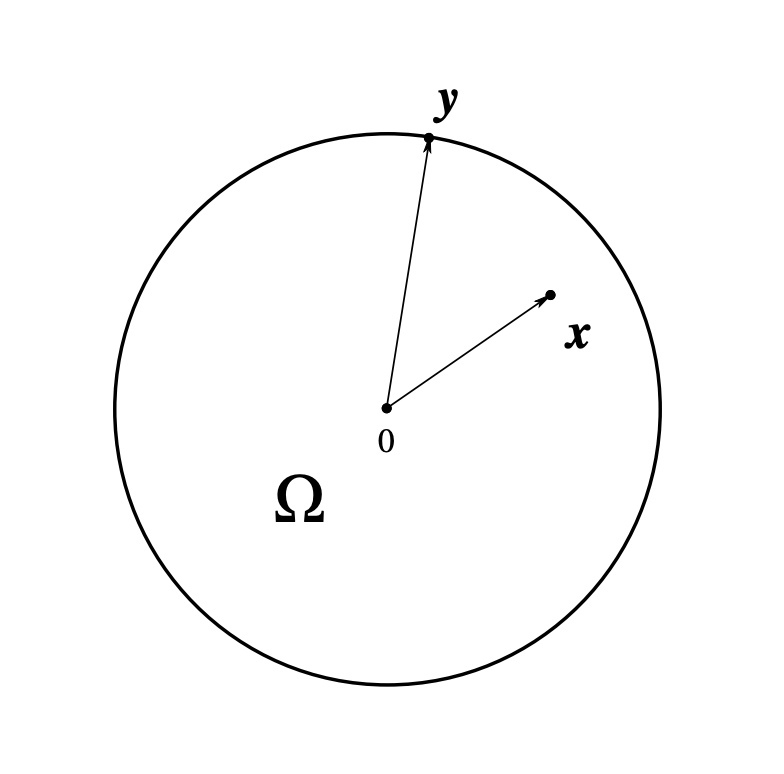
\includegraphics[width = .42\linewidth]{2.jpg}
						\caption[.] {}
					\end{figure}
					\noindent Легко видеть, что расстояние $r$ между $\mathbf{x}$ и $\mathbf{y}$ определяется формулой
					\begin{equation}
						r^2 = | \mathbf{x} - \mathbf{y} |^2 = a^2 - 2ap\cos{(\varphi - \psi)} + \rho^2. \label{35}
					\end{equation}
					Учитывая \ref{35} и выбирая в качестве переменной интегрирования длину дуги $ s = a\psi$, перепишем формулу  \ref{33} в виде:[1]
					\begin{equation}
						u(\mathbf{x}) = \dfrac{1}{2\pi a} \int_{\Gamma_a} \dfrac{(a^2 - \rho^2)}{r^2} g(\mathbf{y}) ds_y = \dfrac{1}{2\pi a} \int_{\Gamma_a} \dfrac{(a^2 - |\mathbf{x}^2|)}{ |\mathbf{x} - \mathbf{y}|^2 } g(\mathbf{y}) ds_y \label{36}
					\end{equation}
					При выполнении лишь условия (i) интеграл Пуассона является гармонической в $\Omega$ функцией, так как этим свойством обладает исходный ряд \ref{25}. То же самое справедливо и для \ref{36}. Более того, если функция $g$ удовлетворяет еще и условию (ii), то можно утверждать, что
					\begin{equation}
						\lim_{\mathbf{x} \rightarrow \mathbf{x}_0} u(\mathbf{x}) = g(\mathbf{x}_0), \:\:\: \lim_{\substack{\rho \rightarrow a \\ \varphi \rightarrow \varphi_0}} u(\rho, \varphi) = g(\varphi_0) \:\:\: \forall \varphi_0 \in [0, 2\pi), \label{37}
					\end{equation}
					так как ряд, из которого получена формула \ref{25} (\ref{36}) является при выполнении условий (i) и (ii) непрерывной функцией в замкнутом круге $\overline{\Omega}$, удовлетворящей граничному условию \ref{2}.
				
					Функция, определенная формулой[2]
					\begin{equation}
						u(\mathbf{x}) = \begin{cases} \dfrac{1}{2\pi a} \int_{\Gamma_a} \dfrac{(a^2-\rho^2)}{|\mathbf{x} - \mathbf{y}|^2} g(\mathbf{y}) ds_y, \mathbf{x} \in \Omega \\ g(\mathbf{x}), \hphantom{\int_{\Gamma_a} \dfrac{(a^2-\rho^2)}{|\mathbf{x} - \mathbf{y}|^2} g(\mathbf{y}) ds_y,}  \mathbf{x} \in \Gamma_a \end{cases} \label{38}
					\end{equation}
					даёт дает решение первой задачи даже в том случае, когда $g$ только непрерывна.
					
					Решение внешней задачи имеет вид
					\begin{equation}
						u(\mathbf{x}) = \begin{cases} \dfrac{1}{2\pi a} \int_{\Gamma_a} \dfrac{(\rho^2-a^2)}{|\mathbf{x} - \mathbf{y}|^2} g(\mathbf{y}) ds_y, \mathbf{x} \in \Omega_e \\ g(\mathbf{x}), \hphantom{\int_{\Gamma_a} \dfrac{(a^2-\rho^2)}{|\mathbf{x} - \mathbf{y}|^2} g(\mathbf{y}) ds_y,}  \mathbf{x} \in \Gamma_a \end{cases}
					\end{equation}
					
					\noindent Рассмотрим доказательство, что \ref{38} дает классическое решение задачи, только при выполнении условия (i) из [1].
					\begin{proof}Для функции $g \equiv 1$ на $\Gamma_a$ решением первой задачи является функция $u \equiv 1$. Это вытекает из принципа максимума. С учетом этого приходим к соотношению 
					\begin{equation}
						1 = \dfrac{1}{2\pi a} \int_{\Gamma_a} \dfrac{a^2 - \rho^2}{r^2} ds_y \label{39}
					\end{equation}			
					\begin{framed}
						\begin{quote}
					\textit{\textbf{Комментарий:}} 
					
					\textit{Принцип максимума: Функция $u$, гармоническая внутри ограниченной области $\Omega$, не может принимать своего максимального и минимального значений внутри $\Omega$, кроме случая, когда $u \equiv \emph{const}$.}\\
						\end{quote}
					\end{framed}
					Умножим обе части на $g(\mathbf{x}_0)$, где $\mathbf{x}_0 \in \Gamma_a$ - фиксированная точка, и вычтем из \ref{36}
					
					\begin{equation}
						u(\mathbf{x}) - g(\mathbf{x}_0) = \dfrac{1}{2 \pi a} \int_{\Gamma_a} [ g(\mathbf{y}) - g(\mathbf{x}_0) ] \dfrac{a^2-\rho^2}{r^2}ds_y. \label{40}
					\end{equation}
					Окружим точку $\mathbf{x}_0$ окружность $S_{2\delta}$ радиуса $2\delta$. $\delta$ выберем таким образом, чтобы во всех точках $\mathbf{y}$ части $\Gamma_1$ границы $\Gamma_a$, лежащей внутри $S_{2\delta}$, выполнялось неравенство
					\begin{equation}
						|g(\mathbf{y}) - g(\mathbf{x}_0)| < \dfrac{\varepsilon}{2}, \label{41}
					\end{equation}
					где $\varepsilon > 0$ -произвольное сколь угодно малое число. 
					
					\begin{figure}[H]
						\centering
						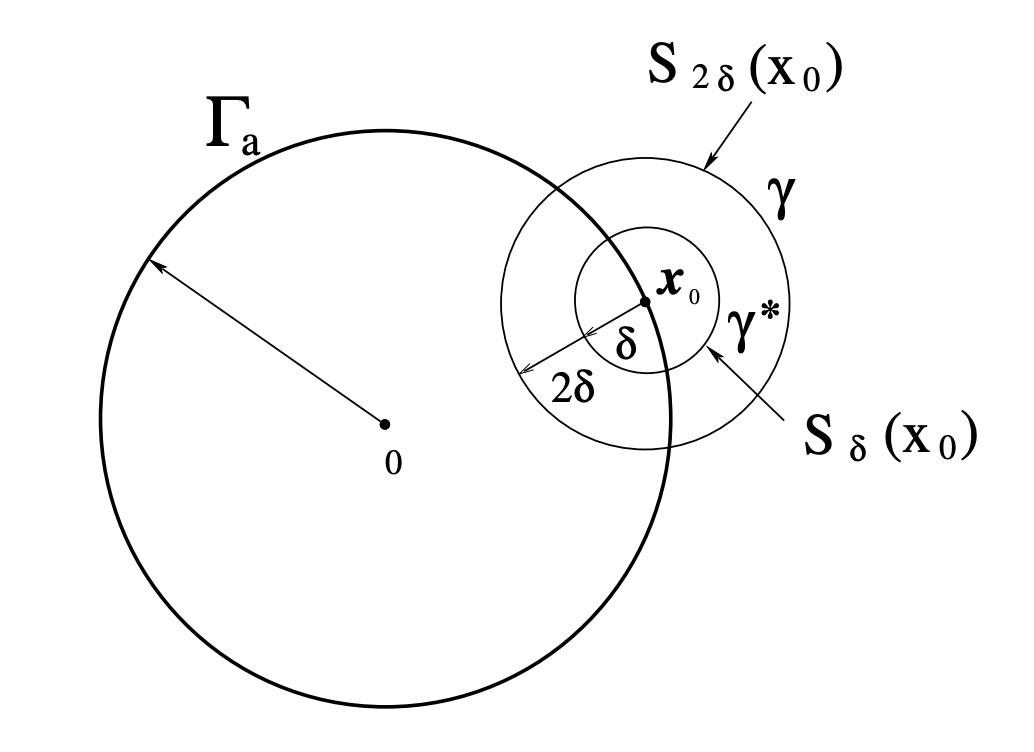
\includegraphics[width = .5\linewidth]{1.jpg}
						\caption[.] {}
					\end{figure}
					
					Положим 
					\begin{equation}
						\Gamma_2 = \Gamma_a \setminus \overline{\Gamma}_1, \:\:\: I_k(\mathbf{x}, \mathbf{x}_0) = \dfrac{1}{2\pi a} \int_{\Gamma_k} [ g({\mathbf{y}}) - g({\mathbf{x}_0}) ] \dfrac{a^2-\rho^2}{r^2} ds_y, \:\:\: k = 1, 2. \label{42}
					\end{equation}
					Из \ref{40} и \ref{42} имеем
					\begin{equation}
						| u(\mathbf{x} - g(\mathbf{x}_0)) | \leq | I_1(\mathbf{x}, \mathbf{x}_0) | +  | I_2(\mathbf{x}, \mathbf{x}_0) | \:\:\: \forall \mathbf{x} \in \Omega
					\end{equation}
					Оценим в отдельности каждое слагаемое в правой части этого неравенства. Учитывая \ref{39} и \ref{41}, имеем 
					\begin{equation}
						| I_1(\mathbf{x}, \mathbf{x}_0) |  < \dfrac{\varepsilon}{2} \dfrac{1}{2\pi a} \int_{\Gamma_1} \dfrac{a^2-\rho^2}{r^2} ds_y < \dfrac{\varepsilon}{2} \dfrac{1}{2\pi a} \int_{\Gamma_a} \dfrac{a^2-\rho^2}{r^2} ds_y = \dfrac{\varepsilon}{2} \:\: \forall \mathbf{x} \in \Omega \label{44}
					\end{equation}
					Оценим теперь $ | I_2(\mathbf{x}, \mathbf{x}_0) | $. Для этого построим еще одну окружность $S_\delta$ с центром в точке $ \mathbf{x}_0 $, имеющую радиус $\delta$. Поскольку нас интересует решение $u(\mathbf{x})$ при $\mathbf{x} \rightarrow \mathbf{x}_0$, то можно считать, что точка $\mathbf{x}$ находится внутри окружности $ S_\delta $. Тогда для любой точки $\mathbf{y} \in \Gamma_2$ выполняется неравенство $ r \equiv | \mathbf{x} - \mathbf{y} | > \delta $. Учитывая, кроме того, что непрерываная на $ [0, 2\pi] $ функция $g$	ограничена, так что $ | g(\mathbf{y}) | \leq M'  = \text{const}$ на $\Gamma_a$, имеем, согласно  \ref{42}, что
					\begin{equation}
						| I_2(\mathbf{x}, \mathbf{x}_0) | \leq \dfrac{2M'(a^2- \rho^2)}{2\pi a\delta^2} \int_{\Gamma_2}ds \leq \dfrac{2M'(a^2- \rho^2)}{\delta^2} \label{45}
					\end{equation}
					Так как число $ \delta $ зафиксировано, а при $\mathbf{x} \rightarrow \mathbf{x}_0$, очевидно, что $ \rho = | \mathbf{x} \rightarrow a | $ и, следовательно, правая часть \ref{45} стремится к нулю, то найдется такое число $\delta_1 > 0$, что выполняется неравенство
					\begin{equation}
							| I_2(\mathbf{x}, \mathbf{x}_0) |  \leq \dfrac{\varepsilon}{2} \:\:\: \text{при} \:\:\:  | \mathbf{x} - \mathbf{x}_0 | < \delta_1. \label{46}
					\end{equation}
					Из \ref{44} и \ref{46} вытекает в силу произвольности $\varepsilon$, что
					\begin{equation}
						| u(\mathbf{x}) - g(\mathbf{x}_0) | \rightarrow 0 \:\:\: \text{при} \:\:\: | \mathbf{x} - \mathbf{x}_0 | \rightarrow 0 \label{47}
					\end{equation}					
					Из \ref{47} , в частности, следует, что $u \in C(\overline{\Omega})$. Кроме того, $ u \in C^2(\Omega) $. Это означает, что формула \ref{38} определяет классическое решение задачи Дирихле.
					\end{proof}
					\section{Заключение}
					Таким образом, с помощью метода Фурье мы получили решения задачи Дирихле уравнения Лапласа в круге и вне круга. Доказали, что они являются классическими решениями, при соблюдении условий (i) и (ii). Затем пребразовали решение к интегралу Пуассона и доказали, что он дает классическое решение, даже в случае соблюдения только условия (i).
					
					\section{Список литературы}
						\begin{enumerate}
							\item Алексеев. Г.В.  Классические модели и методы математической физики. Учебное пособие. -- Владивосток: Дальнаука, 2011. -- 452 c.
							\item Тихонов А.Н., Самарский А.А. Уравнения математической физики: Учебное пособие. -- М. : издательство МГУ, 1999. -- 799 с.
							\item Орловский Д.Г. Уравнение Лапласа в круговых областях[Электронный ресурс] URL: http://www.orlovsky-mephi.narod.ru/Circle.pdf (дата обращение 15.01.2024)
						\end{enumerate}

\end{document}} 
